\documentclass{article}
\usepackage[T1]{fontenc}
\usepackage[utf8]{inputenc}
\usepackage{amssymb}
\usepackage{pythonhighlight}
\usepackage{tikz}
\usepackage{amsmath}
\usepackage[a4paper, left=40mm, right=40mm, top=30mm, bottom=30mm]{geometry}
\usepackage[indent=0pt]{parskip}
\usepackage[backend=biber]{biblatex}
\usepackage{graphicx}
\usepackage{subfig}
\usepackage{subcaption}
\usepackage{float}
\graphicspath{ {../images/} }
\addbibresource{bibliography.bib}

\title{Metody numeryczne - projekt 1 - MACD}
\author{Jerzy Szyjut, numer albumu: 193064}
\date{21.01.2023r.}

\usepackage{csquotes}
\begin{document}

\maketitle

\begin{section}{MACD}
    \subsection{Czym jest MACD?}
    \textbf{MACD} (\textit{Moving Average Convergence/Divergence, pl. zbieżność/rozbieżność średniej kroczącej}) to wskaźnik techniczny, 
    który pomaga identyfikować trendy cenowe i momenty kupna i sprzedaży instrumentów giełdowych. Został on opracowany przez Geralda Appela w 1970 roku.
    Pokazuje on różnicę między dwiema średnimi kroczącymi, zazwyczaj 12-dniową i 26-dniową. Wartość MACD jest różnicą między tymi dwiema średnimi, 
    a sygnał jest 9-dniową średnią kroczącą tej różnicy. Wartość MACD jest obliczana według wzorów:
    \begin{equation}
        EMA_{n} = \alpha \cdot \frac{p_{0} + (1-\alpha) p_{1} + (1-\alpha)^{2} p_{2} + \cdots + (1-\alpha)^{n} p_{n}}{1 + (1-\alpha) + (1-\alpha)^{2} + \cdots + (1-\alpha)^{n}}
    \end{equation}
    \begin{equation}
        MACD = EMA_{12} - EMA_{26}
    \end{equation}
    \begin{equation}
        Signal = EMA_{9}(MACD)
    \end{equation}
    Gdzie:
    \begin{itemize}
        \item $p_{i}$ - cena instrumentu w dniu $i$,
        \item $\alpha = \frac{2}{n+1}$,
        \item $EMA_{n}$ - $n$-dniowa średnia krocząca,
        \item $MACD$ - różnica między dwiema średnimi kroczącymi,
        \item $Signal$ - 9-dniowa średnia krocząca różnicy między dwiema średnimi kroczącymi.
        \item $n$ - liczba dni.
    \end{itemize}
    \subsection{Jak używać MACD?}
    Do analizy wykresu MACD należy użyć dwóch linii: MACD oraz sygnału. Kiedy linia MACD przecina linię sygnału od dołu, jest to sygnał kupna akcji.
    Kiedy linia MACD przecina linię sygnału od góry, jest to sygnał sprzedaży akcji.
\end{section}

\begin{section}{Implementacja wskaźnika MACD dla Nvidia (NVDA)}
    \subsection{Interpretacja wykresów}
    \begin{figure}[H]
        \subfloat[Ceny zamknięcia akcji Nvidia]{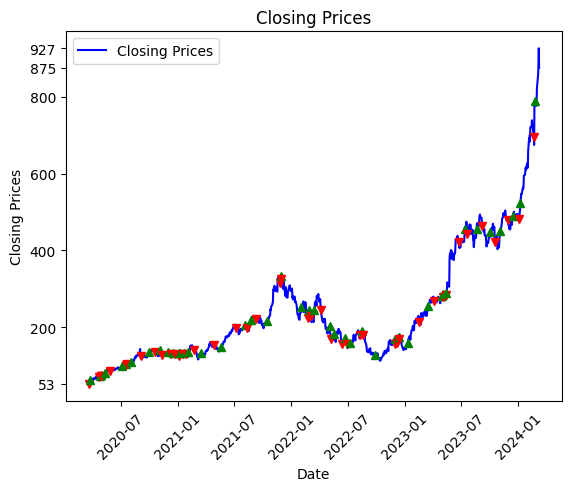
\includegraphics[width=0.5\textwidth]{closing_prices_nvda_normal.png}}
        \subfloat[Wskaźnik MACD dla cen zamknięcia akcji Nvidia]{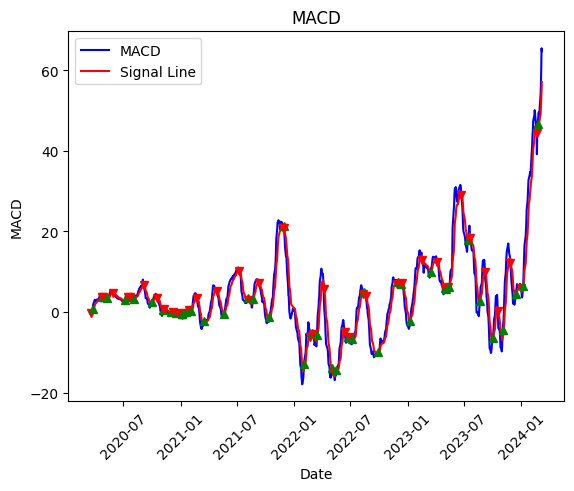
\includegraphics[width=0.5\textwidth]{macd_nvda_normal.png}}
        \caption{Ceny zamknięcia akcji Nvidia oraz wskaźnik MACD z sygnałami kupna/sprzedaży w przedziałach czasowych od 19.03.2020 do 08.03.2024}
    \end{figure}
    Wykresy przedstawiające ceny zamknięcia akcji Nvidia oraz wskaźnik MACD dla tych cen w przedziałach czasowych od 19.03.2020 do 08.03.2024.
    Na przestrzeni tych lat ceny akcji Nvidia wzrosły z 53 do 875 dolarów (wzrost o 1650\%).
    Porównując ten wykres z wykresem wskaźnika MACD, można zauważyć, że wskaźnik MACD proponował sprzedaż w momencie przed lokalnym dołkiem cenowym, a kupno w momencie przed lokalnym szczytem cenowym.
    Wskaźnik MACD przyjmował wartości ujemne, kiedy wartość akcji spadała, a wartości dodatnie, kiedy wartość akcji rosła.
    Dzięki róznicom między wartościami MACD i sygnału, wskaźnik informuje nas o zmianach trendu cenowego.

    \subsection{Interpretacja wycinków wykresów}
    \begin{figure}[H]
        \subfloat[Ceny zamknięcia akcji Nvidia]{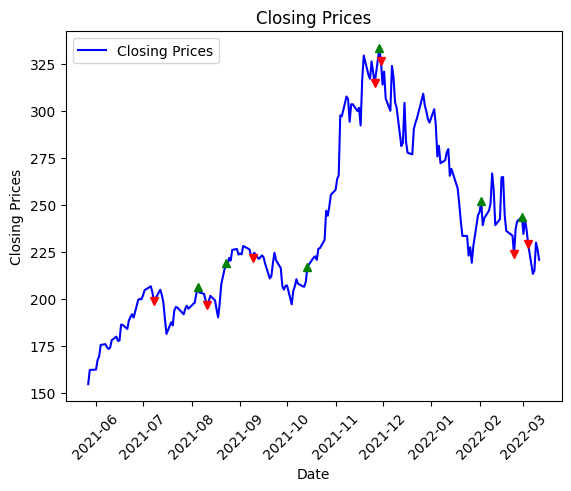
\includegraphics[width=0.5\textwidth]{closing_prices_zoom_nvda_normal.png}}
        \subfloat[Wskaźnik MACD dla cen zamknięcia akcji Nvidia]{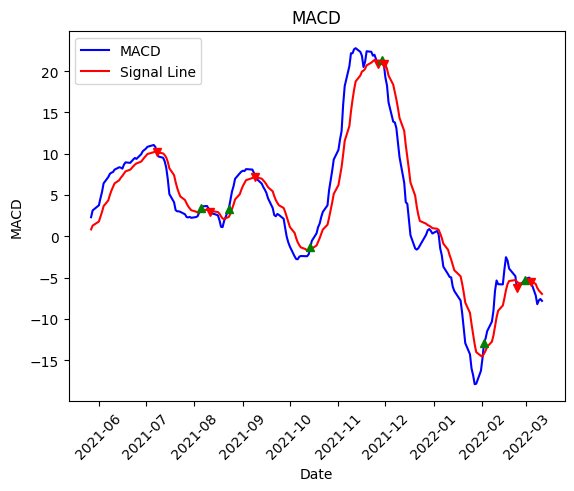
\includegraphics[width=0.5\textwidth]{macd_zoom_nvda_normal.png}}
        \caption{Ceny zamknięcia akcji Nvidia oraz wskaźnik MACD z sygnałami kupna/sprzedaży w okresie od 27.05.2021 do 14.03.2022}
    \end{figure}
    Wycinki wykresów przedstawiające ceny zamknięcia akcji Nvidia oraz wskaźnik MACD w okresie od 27.05.2021 do 14.03.2022.
    Wskaźnik MACD proponował sprzedaż w momencie kiedy na kiedy ceny akcji były rosnące, a kupno w momencie kiedy ceny akcji były spadkowe.
    W przypadku tego okresu wskaźnik MACD był w stanie skutecznie przewidzieć trendy cenowe.

    \begin{figure}[H]
        \subfloat[Ceny zamknięcia akcji Nvidia]{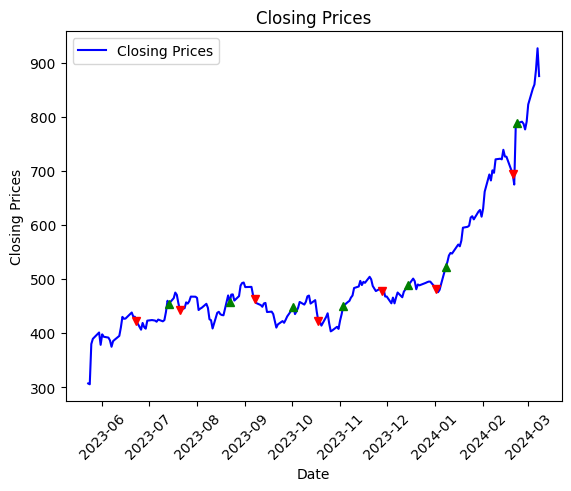
\includegraphics[width=0.5\textwidth]{closing_prices_zoom_2_nvda_normal.png}}
        \subfloat[Wskaźnik MACD dla cen zamknięcia akcji Nvidia]{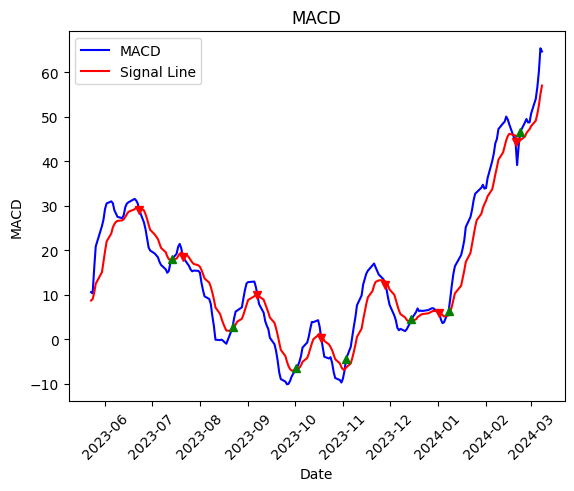
\includegraphics[width=0.5\textwidth]{macd_zoom_2_nvda_normal.png}}
        \caption{Ceny zamknięcia akcji Nvidia oraz wskaźnik MACD z sygnałami kupna/sprzedaży w okresie od 23.05.2023 do 08.03.2024}
    \end{figure}
    Wycinki wykresów przedstawiające ceny zamknięcia akcji Nvidia oraz wskaźnik MACD w okresie od 23.05.2023 do 08.03.2024.
    W tym okresie wskaźnik MACD już nie działał tak skutecznie jak w poprzednim wypadku. Przez częste zmiany trendu cenowego,
    wskaźnik "dawał się łapać" na chwilowe dołki. Jeśli spojrzymy na sygnały kupna/sprzedaży, to widać, że wskaźnik w większości miejsc
    proponował zakup po cenie wyższej niż ostatnia cena sprzedaży i sprzedaż po cenie niższej niż ostatnia cena zakupu.

    \subsection{Wnioski}
    Wskaźnik MACD jest skutecznym narzędziem do analizy trendów cenowych. W przypadku akcji Nvidia, wskaźnik MACD w ogólności był w stanie przewidzieć trendy cenowe.
    Jednak w przypadku częstych zmian trendu cenowego, wskaźnik MACD daje sygnały kupna/sprzedaży, które są nieopłacalne. W okresach w których występując
    częste zmiany trendu cenowego (np. w roku 2020 i pierwszej połowie 2021 roku), wskaźnik MACD często proponuje dokonywanie transakcji, co w prawdziwych 
    warunkach, gdzie nasze transakcje są obarczone prowizjami domów maklerskich, prowadziłoby do straty pieniędzy.
\end{section}

\begin{section}{Algorytm symulujący transakcje na podstawie wskaźnika MACD}
    \begin{figure}[H]
        \centering
        \subfloat[Wykres cen zamknięcia akcji Nvidia]{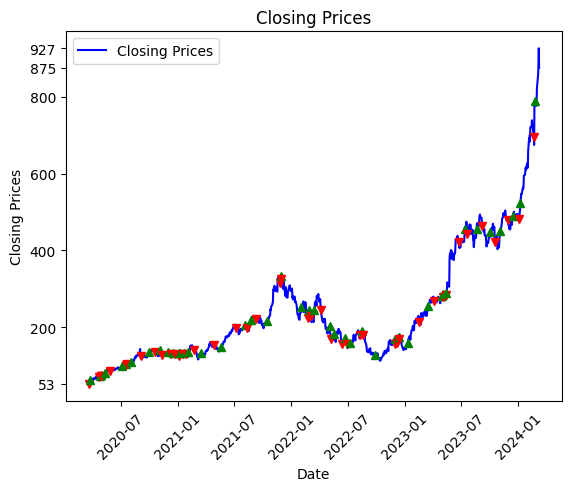
\includegraphics[width=0.5\textwidth]{closing_prices_nvda_normal.png}}
        \subfloat[Wykres wskaźnika MACD dla cen zamknięcia akcji Nvidia]{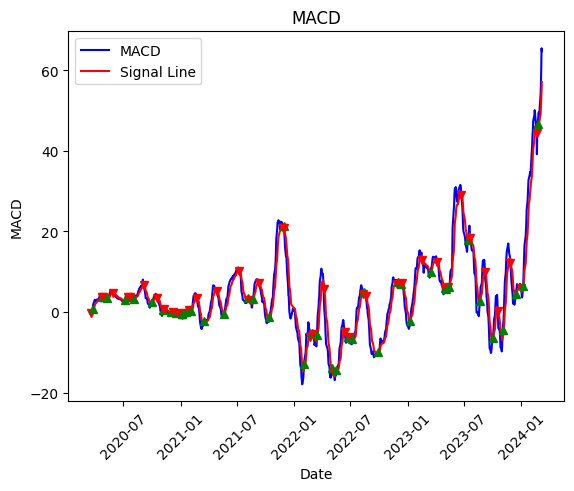
\includegraphics[width=0.5\textwidth]{macd_nvda_normal.png}}
    \end{figure}
    \begin{figure}[H]
        \subfloat[Wykres wartości portfela w zależności od czasu]{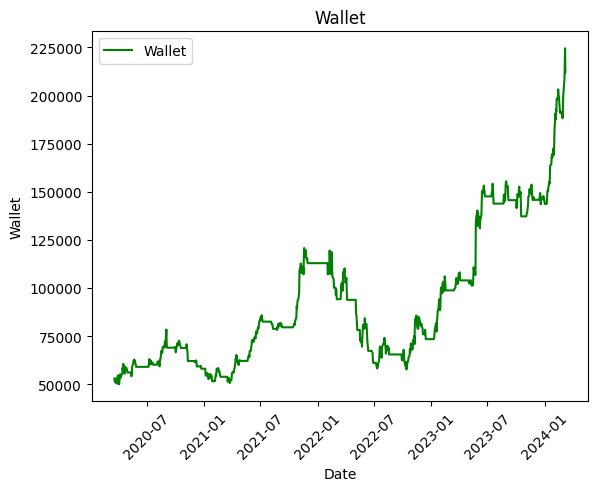
\includegraphics[width=0.5\textwidth]{wallet_nvda_normal.png}}
        \subfloat[Wykres liczby posiadanych akcji w zależności od czasu]{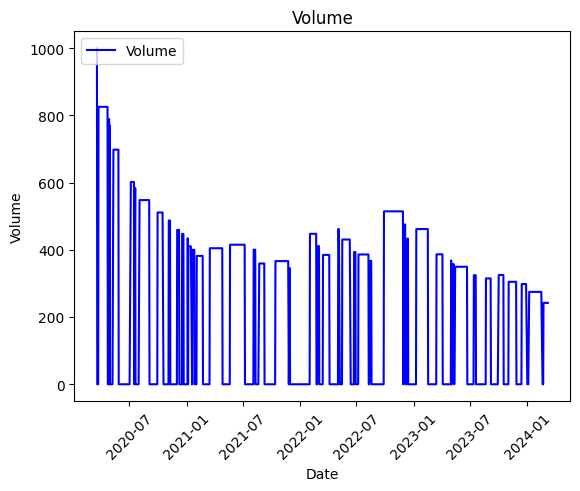
\includegraphics[width=0.5\textwidth]{volume_nvda_normal.png}}
        \caption{Wykresy przedstawiające ceny zamknięcia akcji Nvidia, wskaźnik MACD, wartość portfela oraz liczbę posiadanych akcji na podstawie algorytmu wykorzystującego wskaźnik MACD}
    \end{figure}
    Stworzony przeze mnie algorytm wykupuje akcje za wszystkie swoje pieniądze w momencie kiedy wskaźnik MACD przecina linię sygnału od dołu, 
    a sprzedaje wszystkie swoje akcje w momencie kiedy wskaźnik MACD przecina linię sygnału od góry.
    Algorytm zaczął pracę z 1000 akcjami Nvidia wartymi łącznie 53 092.39 \$, a zakończył z 242 akcjami Nvidia o wartości 212 080.39 \$ co daje 158 988.00 \$ zysku (+399\%).
    Jednak gdybyśmy po prostu zatrzymali te 1000 akcji i sprzedali je na koniec okresu, to zysk wyniósłby 822 187.60 \$ (+1650\%).
\end{section}

\begin{section}{Reverse MACD}
    W trakcie pisania symulacji popełniłem błąd, który spowodował, że ustalałem sygnały kupna i sprzedaży odwrotnie niż powinienem. Co ciekawe, dla instrumentu
    na którym najpierw testowałem algorym - Makarony Polskie S.A. (MAK.PL) ten wskaźnik działał lepiej niż jego podstawowa wersja. Zaczynając z akcjami o wartości 4 174.72zł 
    MACD kończył z 7 375.18 zł (+76\%) a reverse MACD z 9 080.62 zł (+176\%). Dla akcji Nvidia dawał podobne wyniki w dla obu wersji wskaźnika. 
    Zaczynając z akcjami o wartości 53 092.39\$ MACD kończył z 212 080.39\$ (+300\%), 
    a reverse MACD z 211 691.65\$ (+299\%).
    \begin{figure}[H]
        \centering
        \subfloat[Wykres cen zamknięcia akcji Makarony Polskie S.A.]{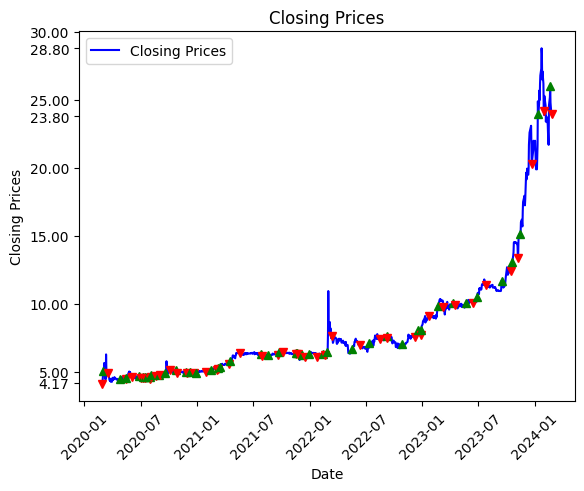
\includegraphics[width=0.5\textwidth]{closing_prices_makarony_normal.png}}
        \subfloat[Wykres wskaźnika MACD dla cen zamknięcia akcji Makarony Polskie S.A.]{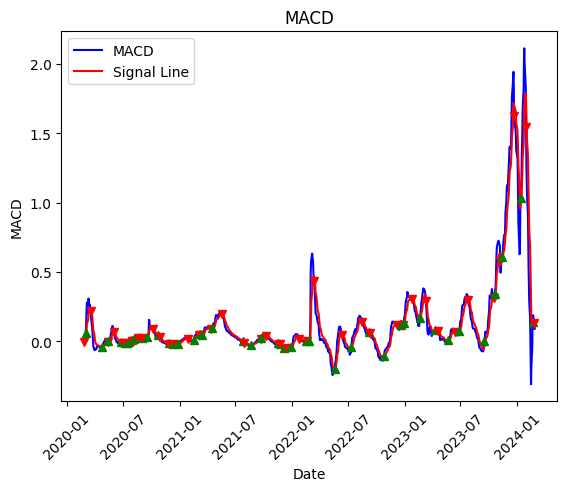
\includegraphics[width=0.5\textwidth]{macd_makarony_normal.png}}
    \end{figure}
    \begin{figure}[H]
        \subfloat[Wykres wartości portfela inwestując w MAK.PL dla MACD w zależności od czasu]{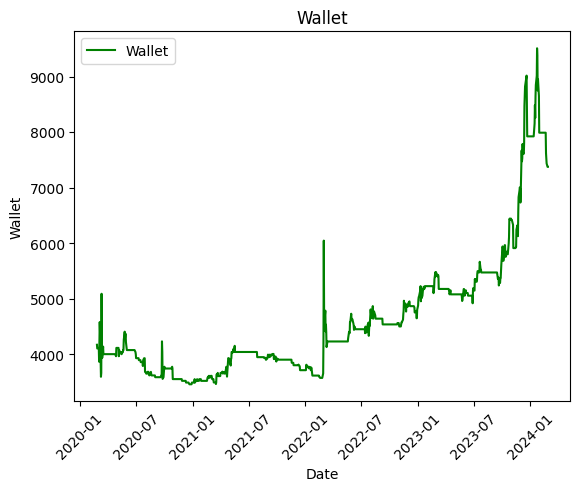
\includegraphics[width=0.5\textwidth]{wallet_makarony_normal.png}}
        \subfloat[Wykres wartości portfela inwestując w MAK.PL dla reverse MACD w zależności od czasu]{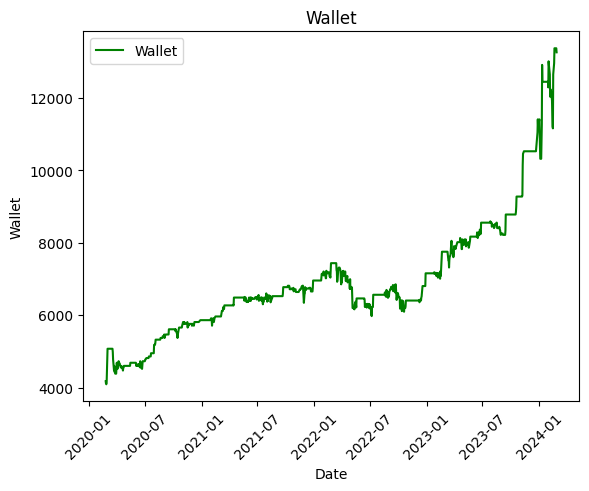
\includegraphics[width=0.5\textwidth]{wallet_makarony_reverse.png}}
    \end{figure}
    \begin{figure}[H]
        \subfloat[Wykres wartości portfela inwestując w NVDA dla MACD w zależności od czasu]{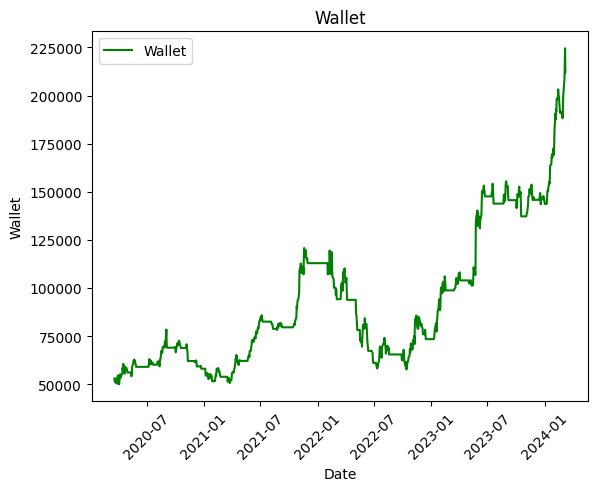
\includegraphics[width=0.5\textwidth]{wallet_nvda_normal.png}}
        \subfloat[Wykres wartości portfela inwestując w NVDA dla reverse MACD w zależności od czasu]{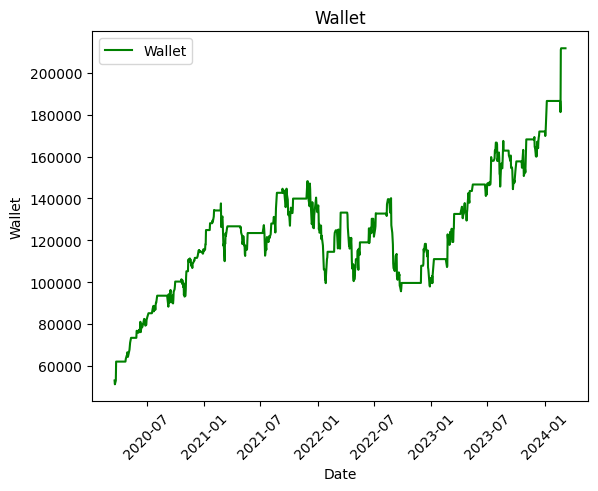
\includegraphics[width=0.5\textwidth]{wallet_nvda_reverse.png}}
        \caption{Wykresy przedstawiające ceny zamknięcia akcji, wskaźnik MACD, wartość portfela inwestując w MAK.PL oraz wartość portfela inwestując w NVDA dla MACD i Reverse MACD}
    \end{figure}
    Dla obu tych instrumentów giełdowych ceny akcji stale rosną, co zapewne powoduje, że wskaźnik MACD daje dochody. Znalazłem więc firmę, której akcje
    spadały w ciągu ostatnich lat, aby sprawdzić, czy MACD lub reverse MACD działają. Wybrałem firmę DoorDash Inc. (DASH), poniżej wykresy.

    \begin{figure}[H]
        \centering
        \subfloat[Wykres cen zamknięcia akcji DoorDash Inc.]{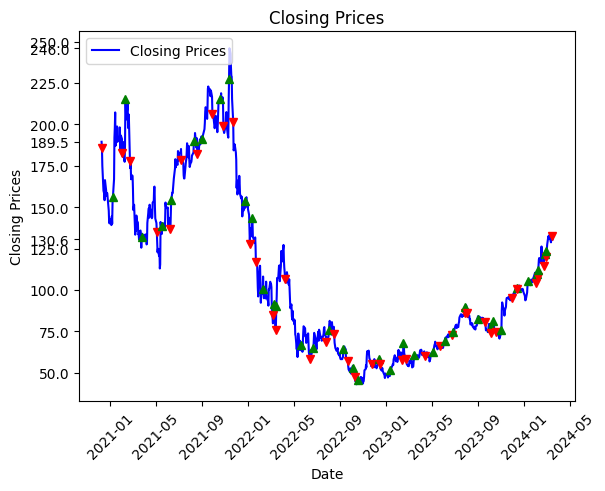
\includegraphics[width=0.5\textwidth]{closing_prices_dash_normal.png}}
        \subfloat[Wykres wskaźnika MACD dla cen zamknięcia akcji DoorDash Inc.]{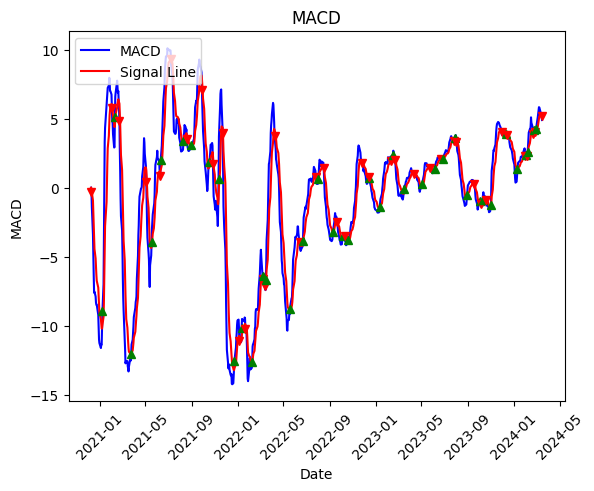
\includegraphics[width=0.5\textwidth]{macd_dash_normal.png}}
    \end{figure}
    \begin{figure}[H]
        \subfloat[Wykres wartości portfela inwestując w DASH dla MACD w zależności od czasu]{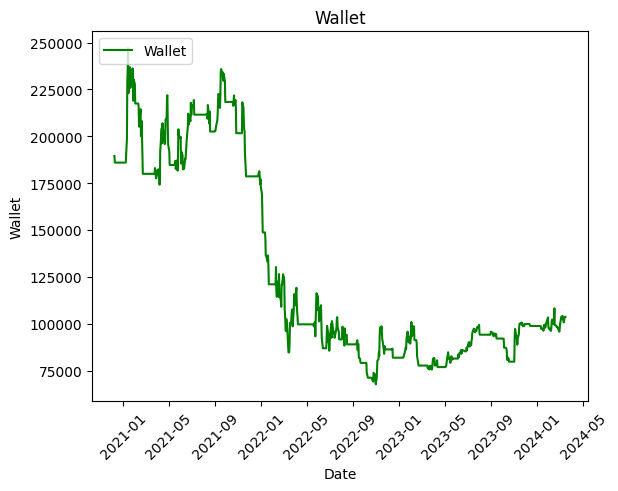
\includegraphics[width=0.5\textwidth]{wallet_dash_normal.png}}
        \subfloat[Wykres wartości portfela inwestując w DASH dla reverse MACD w zależności od czasu]{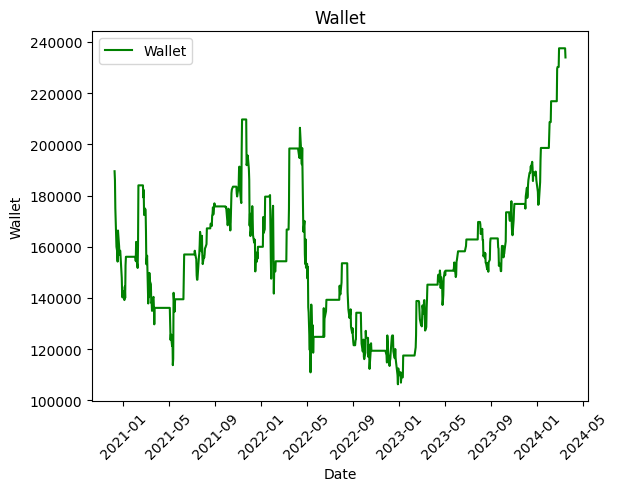
\includegraphics[width=0.5\textwidth]{wallet_dash_reverse.png}}
        \caption{Wykresy przedstawiające ceny zamknięcia akcji, wskaźnik MACD, wartość portfela inwestując w DASH dla MACD i Reverse MACD}
    \end{figure}

    W przypadku akcji DoorDash Inc. (DASH) wskaźnik reverse MACD działał zdecydowanie lepiej niż MACD. Zaczynając z akcjami o wartości 189 510.0 \$
    MACD kończył z 103 791.27 \$ co daje spadek o całe 85 718.72 \$ (-45\%), a reverse MACD kończył z 233 953.18 \$ co daje wzrost o 44 443.18 \$ (+23\%). 
    Akcje DASH spadły w tym okresie o 34\%.
    Dla tego instrumentu giełdowego, którego cena spadała w ciągu ostatnich lat, wskaźnik reverse MACD zadziałał lepiej niż MACD.
\end{section}

\begin{section}{Podsumowanie}
    Na podstawie powyższej analizy i przeprowadzonych symulacji, można stwierdzić, że wskaźnik MACD nie jest najlepszym wskaźnikiem giełdowym.
    W dodatku jego odwrotna wersja działa lepiej lub nieznacznie gorzej dla instrumentów giełdowych, które sprawdzałem. Dla akcji z 
    częstymi zmianami trendu cenowego wskaźnik MACD często zwraca sygnały kupna/sprzedaży, które w prawdziwym życiu,
    w połączeniu z prowizjami domów maklerskich, prowadziłyby do znacznie mniejszych zysków, a nawet straty, poprzez częste transakcje. 
    Wydaje mi się, że ciężko sprawić, aby algorytmu używające po prostu wskaźnika MACD działał lepiej niż strategia "kup i trzymaj".
    Do dalszej analizy warto byłoby sprawdzić czy zmiana długości okresów może poprawić jego skuteczność.
\end{section}

\end{document}